\documentclass[master=cws,masteroption=mmc]{kulemt}
\setup{title={Distributiefunctie van de geometrische normalen gebruiken voor het bouwen van BSP acceleratiedatastructuren},
  author={Jesse Hoobergs},
  promotor={Prof.\,dr.\,ir.\ Philip Dutré},
  assessor={Ir.\,W. Eetveel\and W. Eetrest},
  assistant={Ir.\ M. ~Moulin}}
% De volgende \setup mag verwijderd worden als geen fiche gewenst is.
\setup{filingcard,
  translatedtitle={Using the distribution function of the geometric normals to build BSP acceleration data structures.},
  udc=621.3,
  shortabstract={Hier komt een heel bondig abstract van hooguit 500
    woorden. \LaTeX\ commando's mogen hier gebruikt worden. Blanco lijnen
    (of het commando \texttt{\string\pa r}) zijn wel niet toegelaten!
    \endgraf \lipsum[2]}}
% Verwijder de "%" op de volgende lijn als je de kaft wil afdrukken
%\setup{coverpageonly}
% Verwijder de "%" op de volgende lijn als je enkel de eerste pagina's wil
% afdrukken en de rest bv. via Word aanmaken.
%\setup{frontpagesonly}

% Kies de fonts voor de gewone tekst, bv. Latin Modern
\setup{font=lm}
\setup{inputenc=utf8}

\newcommand\symO{\mathcal{O}}
\newcommand\symSA{\mathcal{SA}}
\newcommand\symSAH{SAH}
\newcommand\symCost{\mathcal{K}}
\newcommand\symLeft{l}
\newcommand\symRight{r}
\newcommand\symNbPrimitives{n}
\newcommand\symIntersection{i}
\newcommand\symTraversal{d}
\newcommand\symTraversalL{\expandafter\MakeUppercase\expandafter{\symTraversal}}
\newcommand\symNodeExample{p}
\newcommand\symLeaf{b}
\newcommand\symLeafL{\expandafter\MakeUppercase\expandafter{\symLeaf}}
\newcommand\symTime{T}
\newcommand\symRender{render}
\newcommand\symTotal{totaal}
\newcommand\symInternal{inwendig}
\newcommand\symBSP{BSP}
\newcommand\symKd{Kd}
\newcommand\symCostTraversalBSP{\symCost_{\symTraversal,\symBSP}}
\newcommand\symCostTraversalKd{\symCost_{\symTraversal,\symKd}}
\newcommand\symCostTraversal{\symCost_{\symTraversal}}
\newcommand\symRandom{random}
\newcommand\symBSPrandom{\symBSP_{\symRandom}}
\newcommand\symBSPrandomkd{\symBSP_{\symRandom+}}
\newcommand\symBSPrandomfastkd{\symBSP^{\symKd}_{\symRandom+}}
\newcommand\symBSPrandomsomekd{\symBSP^{(\symKd)}_{\symRandom+}}
\newcommand\symBSPrandomany{\symBSP^{(\symKd)}_{\symRandom(+)}}
\newcommand\symArbitrary{wn}
\newcommand\symBSParbitrary{\symBSP_{\symArbitrary}}
\newcommand\symBSParbitrarykd{\symBSP_{\symArbitrary+}}
\newcommand\symBSParbitraryfastkd{\symBSP^{\symKd}_{\symArbitrary+}}
\newcommand\symBSParbitrarysomekd{\symBSP^{(\symKd)}_{\symArbitrary+}}
\newcommand\symBSParbitraryany{\symBSP^{(\symKd)}_{\symArbitrary(+)}}
\newcommand\symCluster{cn}
\newcommand\symBSPcluster{\symBSP_{\symCluster}}
\newcommand\symBSPclusterkd{\symBSP_{\symCluster+}}
\newcommand\symBSPclusterfastkd{\symBSP^{\symKd}_{\symCluster+}}
\newcommand\symBSPclustersomekd{\symBSP^{(\symKd)}_{\symCluster+}}
\newcommand\symBSPclusterany{\symBSP^{(\symKd)}_{\symCluster(+)}}
\newcommand\symBSPize{\symBSP_{IZE}}
\newcommand\symBSPizefastkd{\symBSP^{\symKd}_{IZE}}
\newcommand\symBSPKd{\symBSP^{\symKd}}
\newcommand\symBSPsweep{\symBSP_{SWEEP}}
\newcommand\symBSPsweepkd{\symBSP^{\symKd}_{SWEEP}}
\newcommand\symBSPsweepmaybewithkd{\symBSP_{SWEEP(+)}}
\newcommand\symMaxPrims{\symNbPrimitives_{max}}
\newcommand\symMaxDepth{d_{max}}


\newcommand\symBVH{BVH}
\newcommand\symRBSP{RBSP}
\newcommand\symRBSPKd{RBSP^{\symKd}}
\newcommand\symRBSPsomekd{RBSP^{(\symKd)}}
\newcommand\symKDOP{k-DOP}

\newcommand\authorKammaje{Kammaje en Mora}
\newcommand\authorIze{Ize et al}
\newcommand\authorGoldsmithSalmon{Goldsmith en Salmon}
\newcommand\authorMacDonaldBooth{MacDonald en Booth}
\newcommand\authorHavran{Havran}
\newcommand\authorBudge{Budge et al}
\newcommand\authorZachmann{Zachmann}
\newcommand\authorKlosowki{Klosowski et al}
\newcommand\authorHavranBittner{Havran en Bittner}
% Hier kun je dan nog andere pakketten laden of eigen definities voorzien

% Tenslotte wordt hyperref gebruikt voor pdf bestanden.
% Dit mag verwijderd worden voor de af te drukken versie.
\usepackage[pdfusetitle,colorlinks,plainpages=false]{hyperref}

%%%%%%%
% Om wat tekst te genereren wordt hier het lipsum pakket gebruikt.
% Bij een echte masterproef heb je dit natuurlijk nooit nodig!
\IfFileExists{lipsum.sty}%
 {\usepackage{lipsum}\setlipsumdefault{11-13}}%
 {\newcommand{\lipsum}[1][11-13]{\par Hier komt wat tekst: lipsum ##1.\par}}
%%%%%%%

%\includeonly{hfdst-n}
\begin{document}

\begin{preface}
  Dit is mijn dankwoord om iedereen te danken die mij bezig gehouden heeft.
  Hierbij dank ik mijn promotor, mijn begeleider en de voltallige jury.
  Ook mijn familie heeft mij erg gesteund natuurlijk.
\end{preface}

\tableofcontents*

\begin{abstract}
  In dit \texttt{abstract} environment wordt een al dan niet uitgebreide
  samenvatting van het werk gegeven. De bedoeling is wel dat dit tot
  1~bladzijde beperkt blijft.

  \lipsum[1]
\end{abstract}

% Een lijst van figuren en tabellen is optioneel
%\listoffigures
%\listoftables
% Bij een beperkt aantal figuren en tabellen gebruik je liever het volgende:
\listoffiguresandtables
% De lijst van symbolen is eveneens optioneel.
% Deze lijst moet wel manueel aangemaakt worden, bv. als volgt:
\chapter{Lijst van afkortingen en symbolen}
\section*{Afkortingen}
\begin{flushleft}
  \renewcommand{\arraystretch}{1.1}
  \begin{tabularx}{\textwidth}{@{}p{12mm}X@{}}
    LoG   & Laplacian-of-Gaussian \\
    MSE   & Mean Square error \\
    PSNR  & Peak Signal-to-Noise ratio \\
  \end{tabularx}
\end{flushleft}
\section*{Symbolen}
\begin{flushleft}
  \renewcommand{\arraystretch}{1.1}
  \begin{tabularx}{\textwidth}{@{}p{12mm}X@{}}
    42    & ``The Answer to the Ultimate Question of Life, the Universe,
            and Everything'' volgens de \cite{h2g2} \\
    $c$   & Lichtsnelheid \\
    $E$   & Energie \\
    $m$   & Massa \\
    $\pi$ & Het getal pi \\
  \end{tabularx}
\end{flushleft}

% Nu begint de eigenlijke tekst
\mainmatter

\chapter{Inleiding}
\label{hoofdstuk:inleiding}

\section{Fysisch gebaseerd renderen}
\paragraph{Ray tracing}
\textit{Ray tracing} \cite{appel1968some} is een computergrafiek techniek voor fysisch gebaseerd renderen. Het genereert afbeeldingen (= renderen) door stralen te sturen door een scene \cite{Suffern:2007:RTG:1324795}. Een camera wordt op een bepaalde positie in de scene geplaatst en een afbeeldingsvlak, opgedeeld in pixels, wordt ervoor geplaatst. Door elke pixel worden één (of meerdere stralen) gestuurd. Deze stralen worden zichtstralen genoemd en de kleur van hun dichtste intersectiepunt met de scene, bepaalt de kleur van de pixel. Figuur \ref{fig:raytracing} toont dit visueel.\\

\begin{figure}
    \centering
    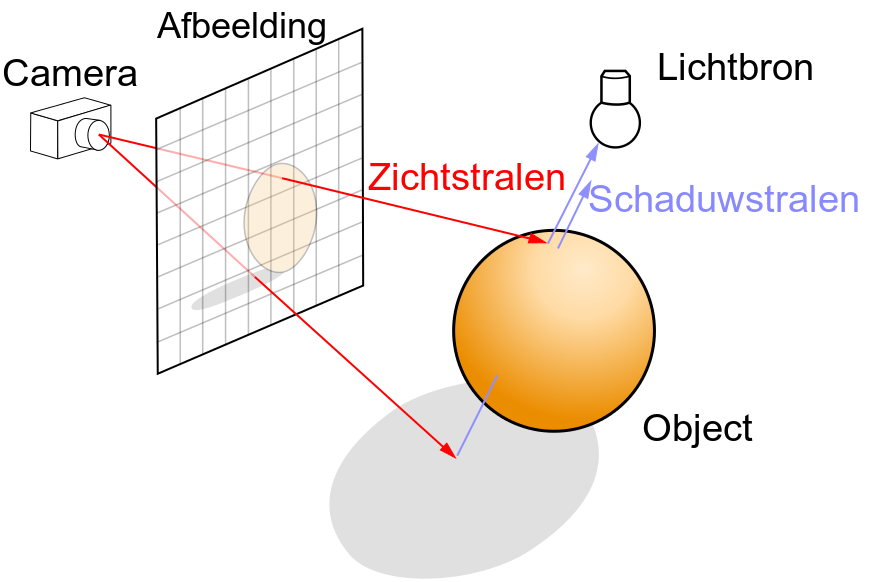
\includegraphics[width=0.5\linewidth]{img/ray-tracing}
    \caption[Visuele voorstelling van \textit{ray tracing}]%
{Visuele voorstelling van \textit{ray tracing} - \small Door elke pixel worden één of meerdere zichtstralen gestuurd. Schaduwstralen worden gebruikt om de belichting in de scene realistisch te maken. Deze afbeelding is een aangepaste versie van een afbeelding op \url{https://en.wikipedia.org/wiki/Ray_tracing_(graphics)}}
    \label{fig:raytracing}    
\end{figure}

Om realistische afbeeldingen te genereren, wordt belichting in het intersectiepunt in rekening gebracht. De eenvoudigste vorm van belichting is directe belichting waarbij een punt donker is als er niet rechtstreeks licht van een lichtbron op valt. Om dit te ondersteunen in \textit{ray tracing} wordt gebruikt gemaakt van schaduwstralen. Dit zijn stralen van het punt naar de lichtbron. Deze schaduwstralen worden geïntersecteerd met de scene, als een intersectiepunt tussen het punt en de lichtbron gevonden wordt, is de lichtbron niet zichtbaar. Bij elke intersectie wordt aan de hand van schaduwstralen gekeken of het punt belicht wordt of niet, als het niet belicht wordt, is de kleur zwart. Voor indirecte belichting - licht dat via reflecties en refracties punten belicht - is \textit{path tracing} \cite{kajiya1986rendering} een veelgebruikte techniek. \textit{Path tracing} reflecteert stralen in het intersectiepunt afhankelijk van het materiaal en als deze straal na een aantal botsingen een lichtbron raakt, krijgt het intersectiepunt een belichting van die lichtbron.    

\paragraph{Acceleratiestructuren}
Het doel van acceleratiestructuren is om de totale tijd nodig om een scene te renderen, te minimaliseren.
Eén van de meest gebruikte representaties van 3D objecten is de \textit{triangle mesh} waarbij het object wordt voorgesteld door een verzameling driehoeken.
De intersectie berekenen tussen een straal en een object komt in dat geval neer op het testen op intersectie tussen de straal en alle driehoeken.
Zelfs een eenvoudige scene kan meer dan honderdduizend driehoeken bevatten en tijdens het renderen kunnen meer dan tien miljoen stralen gestuurd worden.
Het is onhaalbaar om voor elk van deze stralen, elke driehoek op intersectie te testen.
Acceleratiestructuren verminderen de rendertijd door het aantal straal-driehoekintersecties te verminderen.\\

De simpelste acceleratiestructuur bestaat uit het omhullend volume van de scene.
Testen op intersectie met de driehoeken in de scene gebeurt dan enkel als dit omhullend volume intersecteert met de straal.
Deze acceleratiestructuur kan worden uitgebreid tot een boomstructuur door dit volume recursief op te delen in kindvolumes.
Binaire bomen delen elk omhullend volume op in twee nieuwe volumes, andere acceleratiestructuren zoals bijvoorbeeld octrees, delen het volume op in meer dan twee volumes.
\\

Het volume kan worden opgedeeld op twee manieren: volgens objecten of volgens ruimte.
Bij opdeling volgens objecten worden de objecten binnen het volume opgedeeld in meerdere disjuncte groepen en de kindvolumes zijn de omhullende volumes van deze groepen.
Na deze opdeling zit elk object in exact één van deze nieuwe volumes, maar de volumes kunnen overlappen.
Figuur \ref{fig:opdeling-object} toont dit visueel.
Een voorbeeld van een acceleratiestructuur waarbij de opdeling volgens objecten gebeurt is de \textit{Bounding Volume Hierarchy} ($\symBVH$) \cite{goldsmith1987automatic}.
Opdeling volgens ruimte betekent dat de ruimte in het volume wordt opgedeeld in meerdere delen.
Na deze opdeling overlappen deze nieuwe volumes niet, maar een object ligt nu in minstens één (en mogelijks in meerdere) kindvolume(s).
Figuur \ref{fig:opdeling-ruimte} toont dit visueel.
De \textit{Binary Space Partitioning} ($\symBSP$) boom deelt de ruimte van het volume steeds op in twee kindvolumes.
Deze masterproef focust op $\symBSP$ bomen.

\begin{figure}
    \centering
    \begin{subfigure}[t]{0.49\linewidth}
        \centering
    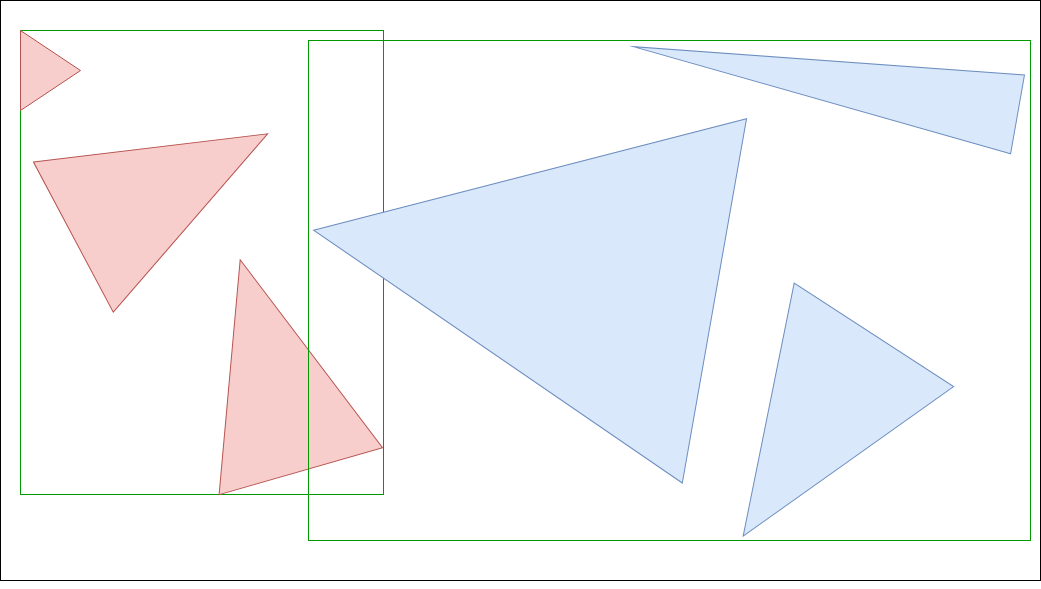
\includegraphics[width=\linewidth]{img/objectSplit}
    \caption{Object}
    \label{fig:opdeling-object} 
    \end{subfigure}
    \begin{subfigure}[t]{0.5\linewidth}
        \centering
    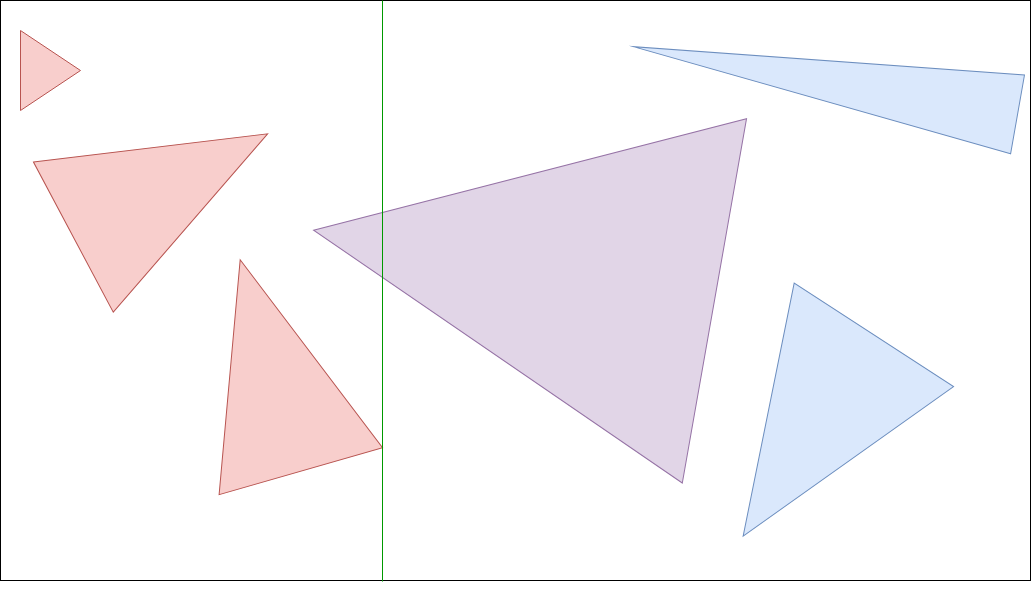
\includegraphics[width=\linewidth]{img/volumeSplit}
    \caption{Ruimte}
    \label{fig:opdeling-ruimte} 
    \end{subfigure}
    \caption[Visuele voorstelling opdeling volume volgens object en ruimte]%
{Visuele voorstelling opdeling volume volgens object en ruimte - \small (a) toont de opdeling volgens object, elk driehoek behoort tot slechts één kindvolume, maar de kindvolumes overlappen. (b) toont de opdeling volgens volume, de paarse driehoek behoort tot beide kindvolumes, maar de kindvolumes zelf zijn disjunct. }
\label{fig:opdeling}
\end{figure}

\section{Doelstelling}
In de praktijk wordt altijd een specifiek soort $\symBSP$ boom gebruikt: de $\symKd$ boom.
Deze boom splitst knopen enkel op via asgealigneerde splitsingsvlakken waardoor hij een aantal computationele voordelen heeft tijdens het bouwen en intersecteren van de boom.
Het nadeel hiervan is dat de $\symKd$ boom zich niet goed kan aanpassen aan complexe niet-asgealigneerde geometrie waardoor bepaalde regio's veel straal-driehoekintersecties nodig hebben.\\

Algemene $\symBSP$ bomen kunnen hiervoor theoretisch gezien een oplossing bieden.
Het ontwerpen van een algemene $\symBSP$ boom die efficiënter is dan de $\symKd$ boom bij het \textit{ray tracen}, is een uitdagend probleem.
Eén van de moeilijkheden bij het bouwen van een algemene $\symBSP$ boom is het kiezen van goede splitsingsvlakken uit het grote aantal mogelijke splitsingsvlakken.
In tegenstelling tot de $\symKd$ boom, waarbij enkel asgealigneerde vlakken mogelijk zijn, zijn alle vlakken mogelijk bij een algemene $\symBSP$ boom.
In deze masterproef wordt onderzocht of het mogelijk is om goede splitsingvlakken te bepalen afhankelijk van de normalen van de driehoeken in de scene.\\

De oplossing die in deze tekst naar voren geschoven wordt, is een nieuw soort algemene $\symBSP$ boom: de $\symBSPsweep$ boom.
De $\symBSPsweep$ boom laat toe om in elke knoop een aantal richtingen te bepalen afhankelijk van de driehoeken in die knoop.
Het beste vlak van alle vlakken met als normaal één van die richtingen, wordt gebruikt om de knoop te splitsen.

\section{Structuur van de tekst}
Hoofdstuk \ref{hoofdstuk:voorgaand-werk} bespreekt de bestaande soorten $\symBSP$ bomen. Hoofdstuk \ref{hoofdstuk:bsp-sweep} start met het beschrijven van het algemene concept van de nieuwe $\symBSPsweep$ boom. Daarna worden drie varianten van dit type boom besproken, één die random richtingen gebruikt en twee die gebruik maken van de normalen. Hoofdstuk \ref{hoofdstuk:implementatie} beschrijft de implementaties, inclusief gelijkenissen en verschillen, van de verschillende bestaande en nieuwe $\symBSP$ bomen. Hoofdstuk \ref{hoofdstuk:resultaten} bespreekt de resultaten van de nieuwe $\symBSPsweep$ bomen in functie van het aantal richtingen en vergelijkt de kwaliteit van de nieuwe bomen met de bestaande $\symBSP$ bomen.

%%% Local Variables: 
%%% mode: latex
%%% TeX-master: "masterproef"
%%% End: 

\chapter{Literatuurstudie}
\label{hoofdstuk:literature}

\section{Raytracing}
Raytracing is een computergraphics techniek om tweedimensionale beelden te genereren van een virtuele driedimensionale wereld bestaande uit driehoeken of andere primitieven.
Door elke pixel worden één (of meerdere) stralen gestuurd vanuit een oogpunt.
Voor elke straal wordt dan de dichtstbijzijnde intersectie met een driehoek in de scene berekend.
De kleur van de pixel is dan het gemiddelde van de kleuren van de straal - driehoek intersectiepunten.

Om deze intersecties efficiënt te kunnen berekenen, wordt gebruik gemaakt van ruimtelijke en/of hiërarchische gegevensstructuren.
De drie hoofdklassen van acceleratie datastructuren in moderne raytracing zijn: Kd-bomen, uniform grid (mogelijks met meerdere niveaus) en as-gealigneerde bounding volume hiërarchieën (BVH). 
Verder wordt het raytracen versneld door: het sturen van pakketten coherente stralen, SIMD extensie van moderne CPU's gebruiken, Bounding Frustrum en interval aritmetica.
Het is nog onduidelijk hoe goed dit voor secundaire stralen werkt ???

Void area: Het verschil tussen de geprojecteerde oppervlakte van het bounding volume en de geprojecteerde oppervlakte van het omhulde object.
Het is aangetoond dat het aantal intersectie testen afhankelijk is van de void oppervlakte. [10]

\section{Binary Space Partitioning bomen}
Binary Space Partitioning bomen of afgekort BSP-bomen splitsen de ruimte op door willekeurig georiënteerde vlakken.
De bounding box van de scene wordt recursief onderverdeeld volgens willekeurige vlakken totdat een bepaalde stopconditie bereikt wordt.
Als enkel as-gealigneerde vlakken gebruikt worden, spreekt men van Kd-bomen.


BSP-bomen zijn in theorie op alle vlakke superieur ten opzicht van Kd-bomen:
\begin{itemize}
	\item De flexibiliteit om splitsingsvlakken te kunnen plaatsen waar ze het meest effectief zijn, zorgt ervoor dat BSP-bomen zich heel goed kunnen aanpassen aan complexe scenes en heel ongelijke scene distributies. Ze zijn robuuster dan Kd-bomen.
	\item Elke Kd-boom kan als een BSP-boom worden uitgedrukt.
\end{itemize}
Een Kd-boom is relatief makkelijk te breken met niet as-gealigneerde geometrie, \cite{Ize} haalt het volgende voorbeeld aan: Neem een smal, lang object, als dit object as-gealigneerd is zal de Kd-boom zeer efficiënt zijn, maar als dit object diagonaal georiënteerd is, zal de kwaliteit van de Kd-boom sterk verminderen.
Voor de BSP-boom - in tegenstelling tot de Kd-boom - zou het roteren geen enkel effect mogen hebben.


Ondanks de theoretische superioriteit worden in de praktijk de Kd-bomen boven de BSP-bomen verkozen.
Er wordt algemeen aangenomen dat BSP-bomen niet bruikbaar zijn omdat ze numeriek instabiel, kostelijk om te doorkruisen en te moeilijk om goed te bouwen zouden zijn.
De numerieke instabiliteit zou volgen uit de beperkte precisie van vlottende komma getallen.  
Het doorkruisen is duurder omdat het berekenen van de afstand van een straal tot een willekeurig vlak een scalair product en een deling vraagt in tegenstelling tot de afstand van een straal tot een as-gealigneerd vlak wat enkel een verschil en een deling vraagt.
Een optimale Kd-boom is - in tegenstelling tot een optimale BSP-boom - niet in staat alle objecten in individuele bladeren onder te verdelen omdat er niet altijd een as-gealigneerd vlak bestaat dat de objecten mooi van elkaar scheidt.  
Dit leidt tot meer straal - object intersectietesten, maar mogelijks wel minder doorkruis stappen.
In het algemeen wordt aangenomen dat het groter aantal intersectietesten wordt goedgemaakt door de snellere doorkruising bij de Kd-boom.
De extra flexibiliteit van de BSP-boom zorgt ervoor dat er $\symO(n^3)$ mogelijke splitsingsvlakken gecontroleerd moeten worden tijdens het bouwproces in tegenstelling tot $6n$ mogelijke splitsingsvlakken bij de Kd-boom.


Ize et al tonen in \cite{Ize} aan dat een algemene BSP-boom even efficiënt en vaak zelfs efficiënter kan zijn dan een Kd-boom om te renderen en dat de snellere doorkruising bij de Kd-boom niet voldoende is om het groter aantal straal - object intersecties goed te maken.
De bouwtijd van de BSP boom is wel een aantal grootteordes groter dan die van de Kd-boom. 

Eén van de optimalisaties die Ize et al doen, is het gebruiken van de goedkopere doorkruis techniek van de Kd-bomen als het splitsingsvlak (toevallig) as-gealigneerd is. 

Restricted Binary Space Partitioning bomen of afgekort RBSP-bomen werden geïntroduceerd door \authorKammaje{ }\cite{Kammaje}.
RBSP-bomen zijn BSP-bomen waarbij de mogelijke splitsingsvlakken beperkt worden tot een kleine verzameling van richtingen voordat de boom geconstrueerd wordt. 
RBSP-bomen lijken op Kd-bomen omdat ze beiden splitsingsvlakken uit een voorafbepaalde verzameling richtingen kiezen.
Tegelijkertijd lijken ze meer op algemene BSP-bomen omdat de vlakken niet as-gealigneerd moeten zijn en het aantal vlakken niet gelimiteerd is tot drie.
De RBSP-boom kan de objecten strakker omhullen en dit zorgt voor minder doorkruisstappen en driehoek intersecties dan Kd-bomen. 
De rendertijd van de RBSP-boom van \cite{Kammaje} was groter dan die van de Kd-boom.
\authorIze{ }zien hiervoor twee mogelijke redenen. 
De eerste reden is dat het doorkruisen van de RBSP-boom te verschillend is van het doorkruisen van de Kd-boom en te duur blijkt te zijn.
Een andere mogelijke reden is dat de RBSP-boom in de lage takken van de boom hetzelfde probleem heeft als de Kd-boom, namelijk dat het niet in staat is om de driehoeken van elkaar af te splitsen.
De rendertijd, aantal node doorkruisingen en aantal driehoek intersecties daalt wel als het aantal splitsingsvlakken stijgt \cite{Kammaje}.
\authorKammaje{ }observeerden experimenteel een complexiteit van $\symO(m^{1.6}*n*log^2(n))$ voor het bouw algoritme met $m$ het aantal splitsingsassen $n$ het aantal driehoeken.
Budge (\cite{Budge}) optimaliseerde het bouwen en doorkruisen van RBSP-bomen.

De manier waarop een node uiteindelijk wordt opgedeeld in twee delen kan een grote impact hebben op het aantal doorkruisstappen en driehoek intersecties.
Voor een Kd-boom is de Surface Area Heuristiek (SAH) de beste gekende methode om bomen met minimale verwachtte kost te bouwen.
De SAH schat de kost van een splitsingsvlak door te veronderstellen dat beide helften bladeren worden. 
De verwachte kost om een node {\symNodeExample} te splitsen in nodes ${\symLeft}$ en ${\symRight}$ is dan: $\symCost_\symNodeExample = \frac{\symSA(\symLeft)}{\symSA(\symNodeExample)}*\symNbPrimitives_\symLeft*\symCost_\symIntersection + \frac{\symSA(\symRight)}{\symSA(\symNodeExample)}*\symNbPrimitives_\symRight*\symCost_\symIntersection + \symCost_\symTraversal$ met kost $\symCost$, oppervlakte $\symSA()$ en aantal driehoeken $\symNbPrimitives$.
De subscripts ${\symIntersection}$ en ${\symTraversal}$ staan voor respectievelijk intersectie en doorkruising.
\authorKammaje{ }toonden aan hoe de SAH aangepast kan worden voor RBSP-bomen \cite{Kammaje}. 
\authorIze{ }toonden aan dat dezelfde theorie ook werkt voor algemene BSP-bomen \cite{Ize}.

Het bouwen van een BSP-boom is heel gelijkaardig aan het bouwen van een Kd-boom \cite{Ize}. 
Er moet wel meer rekening gehouden worden met de verminderde numerieke precisie. 
Het berekenen van de oppervlakte van een node moet ook aangepast worden naar de berekening van de oppervlakte van een veelvlak (meer bepaald een polytoop) in tegenstelling tot de oppervlakte van een as-gealigneerde box.
Bepalen welke willekeurige splitsingsvlakken gebruikt worden, vraagt ook extra aandacht.

Om de SAH te kunnen berekenen moet de oppervlakte van de nodes gekend zijn. 
Voor een Kd-boom is dit triviaal te berekenen maar bij een BSP-boom wordt een node gedefinieerd als de intersectie van halfruimtes.
\authorKammaje{ }vormen eerst de polytoop door de vorige polytoop te clippen met het splitsingsvlak en sommeren daarna de oppervlaktes van de zijvlakken \cite{Kammaje}.
\authorIze{ }gebruiken dezelfde methode voor de BSP-boom \cite{Ize}.
De methode om deze nieuwe polytoop te berekenen moet robuust zijn en zeer smalle polytopen aankunnen.
\authorKammaje{ }spreken ook over een tweede methode die gebruik maakt van het feit dat de oppervlakte kwadratisch varieert tussen elke twee opeenvolgend geprojecteerde punten van de pqolyhedron volgens een de as. 

Deze methode zou iets sneller zijn, maar er wordt weinig uitleg gegeven over de exacte berekeningen.

Numerieke inprecisie maakt het moeilijk om te bepalen of een punt exact op een vlak ligt -> er moet gebruik gemaakt worden van een epsilon, die groot genoeg moet zijn, maar ook niet te groot.\cite{Ize}.  

\authorIze{ }moeten een aanpassing maken aan de SAH omdat ze twee verschillende doorkruis kosten hebben: $\symCostTraversalBSP$ en $\symCostTraversalKd$.
Als ze deze rechtstreeks in de SAH gebruiken, leidt dit tot overmatig gebruik van BSP nodes ten opzichte van Kd nodes, zelfs wanneer $\symCostTraversalBSP$ vele malen groter dan $\symCostTraversalKd$ wordt gezet.
De reden hiervoor is de veronderstelling dat een split bladeren genereert met een kost die lineair is in het aantal driehoeken.
Dit werkt goed als er maar één doorkruis kost is, omdat de doorkruis kost enkel beïnvloedt of de node gesplitst wordt of niet.
In \cite{Ize} bepaald de doorkruis kost niet alleen of er gesplitst moet worden, maar ook of de kostelijker te doorkruisen BSP split te verkiezen is boven de goedkopere Kd split.
De lineaire intersectie kost zal snel de constante doorkruis kost overstijgen waardoor de optimale split uiteindelijk bijna volledig gebaseerd zal zijn op welke split resulteert in minder driehoek intersectie testen.
Om dit op te lossen, laten ze $\symCostTraversalBSP$ lineair variëren met het aantal driehoeken: $\symCostTraversalBSP = \alpha * \symCost_\symIntersection * (\symNbPrimitives - 1) + \symCostTraversalKd$. waarbij $\alpha$ een instelbare parameter is. \authorIze{ }gebruiken 0.1 als waarde voor $\alpha$.
Als er na het evalueren van alle splitsingsvlakken geen splitsingsvlak gevonden is dat de kost kleiner maakt dan de kost om een blad node te maken, worden alle BSP splitsingsvlakken opnieuw geëvalueerd maar nu met een vaste kost.

Bij elke node moet beslist worden voor welke vlakken de SAH geëvalueerd wordt. Havran (!!cite) toonde aan dat voor Kd-bomen enkel de splitsingsvlakken rakend aan de driehoeken bekeken moesten worden.
Voor elke driehoek zijn er maar 6 vlakken die aan die voorwaarde voldoen, waardoor er maar $\symO(n)$ kandidaat splitsingsvlakken zijn per node.
Dit resultaat rechtstreeks uitbreiden naar de BSP-boom resulteert in $\symO(n^3)$ of meer kandidaat splitsingsvlakken per node wat vaak praktisch onmogelijk is. 
\authorIze{ }beperken zichzelf tot slechts $\symO(n)$ kandidaat splitsingsvlakken per node. 
Dit zorgt ervoor dat de bouwtijd praktisch blijft, maar heeft als nadeel dat ze mogelijke betere splitsingsvlakken niet bekijken.
Voor elke driehoek in een node bekijken ze: het vlak van de driehoek zelf (auto-partitie), de drie vlakken loodrecht op de driehoek door de zijdes en de standaard zes as-gealigneerde vlakken die door de Kd-boom gebruikt worden.
De eerste vier vlakken zouden niet mogelijk zijn bij een RBSP-boom omdat een RBSP-boom op voorhand vastlegt welke splitsingsvlakken voor elke node bekeken worden, ongeacht de driehoeken in die node.

Een Kd-boom kan gebouwd worden in $\symO(n*log(n))$ volgens Wald en Havram [22].
Dit is niet mogelijk voor de BSP-boom omdat we de driehoeken volgens een willekeurige richting moeten opdelen.
De standaard $\symO(n^2)$ Kd-boom bouw methode kan wel gebruikt worden.
Omdat de test vlakken niet gesorteerd kunnen worden, is het niet mogelijk om snellere en met lagere complexiteit te bouwen.
\authorIze{ }verlaagt de complexiteit door gebruik te maken van een hulp gegevensstructuur om het aantal driehoeken te tellen die links van, op en rechts van het vlak liggen.
Deze structuur is een bounding sphere hiërarchie over de driehoeken waarbij elke node bijhoudt hoeveel driehoeken hij bevat. 
Op deze manier kan het aantal driehoeken direct gevonden worden als een node volledig aan één kant van het vlak ligt.
Deze structuur wordt via het standaard as-gealigneerde BVH algoritme gebouwd, wat heel snel is in verhouding tot de BSP bouwtijd.
In het slechtste geval (als alle driehoeken op het splitsingsvlak liggen), moeten alle bladeren bekeken worden en wordt lineaire tijd gebruikt voor dit splitsingsvlak. 
Deze slechtste geval complexiteit verhoogt de bouwtijd niet omdat we sowieso lineaire tijd nodig hebben om te tellen, in het algemeen zorgt deze hulp structuur voor een sub kwadratische bouwtijd.
Deze structuur moet na elke split geüpdatet worden en dit kost $\symO(n)$, maar aangezien er toch $\symO(n)$ splitsingsvlakken getest worden, verhoogd dit de complexiteit niet. 

Een straal doorkruist een Kd-boom door de intersectie te berekenen van de straal en het splitsingsvlak.  
Deze intersectie geeft een straal afstand to het vlak waarmee de straal opgedeeld kan worden in verschillende segmenten.
Het initiële segment wordt berekend door de straal te clippen met de as-gealigneerde bounding box. 
Een node wordt doorkruist als het segment van de straal, de node overlapt.
Omdat de twee kindknopen van een node nooit overlappen, kan makkelijk bepaald worden welk kind dichter bij de oorsprong van de straal ligt en kan die knoop eerst doorkruist worden (als die tenminste het segment van de straal overlapt), hierdoor kan het doorkruisen van de tweede kindknoop mogelijks sneller beëindigd worden. 

Het algoritme om een BSP-boom te doorkruisen is hetzelfde als dat om de Kd-boom te doorkruisen met twee wijzigingen.
De eerste wijziging is dat het berekenen van de afstand tot het vlak nu twee scalaire producten en een vlottende komma deling in tegenstelling tot een verschil en een vermenigvuldiging met een vooraf berekende inverse.
De tweede wijzing volgt uit de beperkte precies van vlotte komma getallen waardoor de opgeslagen normalen van willekeurige vlakken altijd licht zullen afwijken van de echte waarde.
Hierdoor kunnen we niet rechtstreeks de berekende waarde voor de afstand gebruiken, maar moeten we veronderstellen dat alle afstanden kleiner dan een bepaalde epsilon, aan eender welke kant van het vlak kan liggen en dus moeten we beide nodes doorkruisen.
\authorIze{ }ondervonden dat de BSP doorkruising 75\% trager is dan een Kd doorkruising, dit is vooral door de twee scalaire producten en de deling.
Daarom gebruiken ze een hybride aanpak waarbij de as-gealigneerde splitsingen gebruik maken van de Kd doorkruising.
Het originele straal segment clippen ze net zoals bij de Kd-boom met de originele as-gealigneerde bounding box.
Dit heeft als voordeel dat het stralen die het hele object missen, zeer snel kan afwijzen. 
\authorKammaje{ }gebruikten een complexer bounding volume.

\authorIze{ }maken gebruik van Traversal Based Triangle Intersection wat de meeste expliciete straal - driehoek intersectietesten overbodig maakt.

\subsection{Een item}

\section{Besluit van dit hoofdstuk}

\chapter{Het eerste hoofdstuk}
\label{hoofdstuk:1}
Een hoofdstuk behandelt een samenhangend geheel dat min of meer op zichzelf
staat. Het is dan ook logisch dat het begint met een inleiding, namelijk
het gedeelte van de tekst dat je nu aan het lezen bent.

\section{Eerste onderwerp in dit hoofdstuk}
De inleidende informatie van dit onderwerp.

\subsection{Een item}
De bijbehorende tekst. Denk eraan om de paragrafen lang genoeg te maken en
de zinnen niet te lang.

Een paragraaf omvat een gedachtengang en bevat dus steeds een paar zinnen.
Een paragraaf die maar \'e\'en lijn lang is, is dus uit den boze.

\section{Tweede onderwerp in dit hoofdstuk}
Er zijn in een hoofdstuk verschillende onderwerpen. We zullen nu
veronderstellen dat dit het laatste onderwerp is.

\subsection{Een item}
Maak ook geen misbruik van opsommingen. Voor korte opsommingen gebruik je
geen ``\verb|itemize|'' of ``\texttt{enumerate}'' commando's. Doe dus
\emph{niet} het volgende:
\begin{quote}
  De Eiffeltoren bevat drie verdiepingen:
  \begin{itemize}
  \item de eerste;
  \item de tweede;
  \item de derde.
  \end{itemize}
\end{quote}
Maar doe:
\begin{quote}
  De Eiffeltoren bevat drie verdiepingen: de eerste, de tweede en de derde.
\end{quote}

\section{Besluit van dit hoofdstuk}
Als je in dit hoofdstuk tot belangrijke resultaten of besluiten gekomen
bent, dan is het ook logisch om het hoofdstuk af te ronden met een
overzicht ervan. Voor hoofdstukken zoals de inleiding en het
literatuuroverzicht is dit niet strikt nodig.

%%% Local Variables: 
%%% mode: latex
%%% TeX-master: "masterproef"
%%% End: 

\chapter{Een volgend hoofdstuk}
\label{hoofdstuk:2}
Een hoofdstuk behandelt een samenhangend geheel dat min of meer op zichzelf
staat. Het is dan ook logisch dat het begint met een inleiding, namelijk
het gedeelte van de tekst dat je nu aan het lezen bent.

\section{Eerste onderwerp in dit hoofdstuk}
De inleidende informatie van dit onderwerp.

\subsection{Een item}
Een tekst staat nooit alleen. Dit wil zeggen dat er zeker ook referenties
nodig zijn. Dit kan zowel naar on-line documenten\cite{wiki} als naar
boeken\cite{pratchett06:_good_omens}.

\section{Figuren}
Figuren worden gebruikt om illustraties toe te voegen. Dit is dan ook de
manier om beeldmateriaal toe te voegen zoals getoond wordt in
figuur~\ref{fig:logo}.

\begin{figure}
  \centering
  
\includegraphics{logokul}
  \caption{Het KU~Leuven logo.}
  \label{fig:logo}
\end{figure}

\section{Tabellen}
Tabellen kunnen gebruikt worden om informatie op een overzichtelijke te
groeperen. Een tabel is echter geen rekenblad! Vergelijk maar eens
tabel~\ref{tab:verkeerd} en tabel~\ref{tab:juist}. Welke tabel vind jij het
duidelijkst?

\begin{table}
  \centering
  \begin{tabular}{||l|lr||} \hline
    gnats     & gram      & \$13.65 \\ \cline{2-3}
              & each      & .01 \\ \hline
    gnu       & stuffed   & 92.50 \\ \cline{1-1} \cline{3-3}
    emu       &           & 33.33 \\ \hline
    armadillo & frozen    & 8.99 \\ \hline
  \end{tabular}
  \caption{Een tabel zoals het niet moet.}
  \label{tab:verkeerd}
\end{table}

\begin{table}
  \centering
  \begin{tabular}{@{}llr@{}} \toprule
    \multicolumn{2}{c}{Item} \\ \cmidrule(r){1-2}
    Animal    & Description & Price (\$)\\ \midrule
    Gnat      & per gram    & 13.65 \\
              & each        & 0.01 \\
    Gnu       & stuffed     & 92.50 \\
    Emu       & stuffed     & 33.33 \\
    Armadillo & frozen      & 8.99 \\ \bottomrule
  \end{tabular}
  \caption{Een tabel zoals het beter is.}
  \label{tab:juist}
\end{table}

\section{Lorem ipsum}
Tenslotte gaan we hier nog wat tekst voorzien zodat er minstens een
bijkomende bladzijde aangemaakt wordt. Dat geeft de gelegenheid om eens te
zien hoe de koptekst en de voettekst zich gedragen.

\subsection{Lorem ipsum dolor sit amet, consectetur adipiscing elit}
Sed nec tortor id felis tristique sodales. Nulla nec massa eu dui fermentum
tincidunt. Integer ullamcorper ante eget eros posuere faucibus. Nam id
ligula ut augue pulvinar vulputate id at purus. Aenean condimentum tortor
eu mi placerat eget eleifend massa mollis. Nam est mi, sagittis quis
euismod eget, sagittis in nibh. Proin elit turpis, aliquam et imperdiet
sed, volutpat eu turpis.

Pellentesque vel enim tellus, vitae egestas turpis. Praesent malesuada elit
non nisi sollicitudin non blandit lacus tincidunt. Morbi blandit urna at
lectus ornare laoreet. Suspendisse turpis diam, lobortis dictum luctus
quis, commodo at lorem. Integer lacinia convallis ultricies. Sed quis augue
neque, eu malesuada arcu. Nullam vehicula, purus vitae sagittis pulvinar,
erat eros semper massa, eu egestas nibh erat quis magna. Cras pellentesque,
nisl eu dapibus volutpat, urna augue ornare quam, quis egestas lectus nulla
a lectus.

Vivamus dictum libero in massa cursus sed vulputate eros imperdiet. Donec
lacinia, libero ac lobortis egestas, nibh dui ornare arcu, luctus porttitor
velit massa sit amet quam. Maecenas scelerisque laoreet diam, vitae congue
quam adipiscing vitae. Aliquam cursus nisl a leo convallis eleifend
fermentum massa porta. Nunc libero quam, dapibus dapibus molestie sit amet,
faucibus vel nunc.

\subsection{Praesent auctor venenatis posuere}
Sed tellus augue, molestie in pulvinar lacinia, dapibus non ipsum. Fusce
vitae mi vitae enim ullamcorper hendrerit eu malesuada est. Proin iaculis
ante sed nibh tincidunt vel interdum libero posuere. Vivamus accumsan metus
quis felis congue suscipit dapibus enim mattis. Fusce mattis tortor eget
ipsum interdum sagittis auctor id metus.

Integer diam lacus, pharetra sit amet tempor et, tristique non lorem.
Aenean auctor, nisi eu interdum fermentum, lectus massa adipiscing elit,
sed facilisis orci odio a lectus. Proin mi nibh, tempus quis porta a,
viverra quis enim. In sollicitudin egestas libero, quis viverra velit
molestie eget. Nulla rhoncus, dolor a mollis vestibulum, lacus elit semper
nisi, nec sollicitudin sem urna eu magna. Nunc sed est urna, euismod congue
mi.

\subsection{Cras vulputate ultricies venenatis}
Vivamus eros urna, sodales accumsan semper vel, lobortis sit amet mauris.
Etiam condimentum eleifend lorem, ullamcorper ornare lectus aliquet vitae.
Praesent massa enim, interdum sit amet semper et, venenatis ut elit.
Quisque faucibus, quam ac lacinia imperdiet, nulla neque elementum purus,
tempus rutrum justo massa porta sapien. Vestibulum ante ipsum primis in
faucibus orci luctus et ultrices posuere cubilia Curae; Sed ultrices
interdum mi, et rhoncus sapien rutrum sed.

Duis elit orci, molestie quis sollicitudin sed, convallis non ante.
Maecenas tincidunt condimentum justo, et ultricies leo tristique vitae.
Vestibulum quis quam non lectus dapibus eleifend a vitae nibh. Nam nibh
justo, pharetra quis iaculis consequat, elementum quis justo. Etiam mollis
lacinia lacus, nec sollicitudin urna lobortis ac. Nulla facilisi.

Proin placerat risus eleifend erat ultricies placerat. Etiam rutrum magna
nec turpis euismod consectetur. Phasellus tortor odio, lacinia imperdiet
condimentum sed, faucibus commodo erat. Phasellus sed felis id ante
placerat ultrices. Aenean tempor justo in tortor volutpat eu auctor dolor
mollis. Aenean sit amet risus urna. Morbi viverra vehicula cursus.

\subsection{Donec nibh ante, consectetur et posuere id, tempus nec arcu}
Curabitur a tellus aliquet ipsum pellentesque scelerisque. Etiam congue,
risus et volutpat rutrum, est purus dapibus leo, non cursus metus felis
eget ligula. Vivamus facilisis tristique turpis, ut pretium lectus luctus
eleifend. Fusce magna sapien, ullamcorper vitae fringilla id, euismod quis
ante.

Phasellus volutpat, nunc et pharetra semper, sem justo adipiscing mauris,
id blandit magna quam et orci. Vestibulum a erat purus, ut molestie ante.
Vestibulum ante ipsum primis in faucibus orci luctus et ultrices posuere
cubilia Curae; Proin turpis diam, consequat ut ullamcorper ut, consequat eu
orci. Sed metus risus, fringilla nec interdum vel, interdum eu nunc.
Suspendisse vel sapien orci.

\subsection{Morbi et mauris tempus purus ornare vehicula}
Mauris sit amet diam quam, eget luctus purus. Sed faucibus, risus semper
eleifend iaculis, mi turpis bibendum nisl, quis cursus nibh nisl sit amet
ipsum. Vestibulum tempor urna vitae mi auctor malesuada eget non ligula.
Nullam convallis, diam vel ultrices auctor, eros eros egestas elit, sed
accumsan arcu tortor eget leo. Vestibulum orci purus, porttitor in pharetra
eget, tincidunt eget nisl. Nullam sit amet nulla dui, facilisis vestibulum
dui.

Donec faucibus facilisis mauris ac cursus. Duis rhoncus quam sed nisi
laoreet eu scelerisque massa tincidunt. Vivamus sit amet libero nec arcu
imperdiet tempor quis non libero. Sed consequat dignissim justo. Phasellus
ullamcorper, velit quis posuere vulputate, felis erat tincidunt mauris, at
vestibulum justo lectus et turpis. Maecenas lacinia convallis euismod.
Quisque egestas fermentum sapien eu dictum. Sed nec lacus in purus dictum
consequat quis vel nisl. Fusce non urna sem. Curabitur eu diam vitae elit
accumsan blandit. Nullam fermentum nunc et leo dictum laoreet. Donec semper
varius velit vel fringilla. Vivamus eu orci nunc.

\section{Besluit van dit hoofdstuk}
Als je in dit hoofdstuk tot belangrijke resultaten of besluiten gekomen
bent, dan is het ook logisch om het hoofdstuk af te ronden met een
overzicht ervan. Voor hoofdstukken zoals de inleiding en het
literatuuroverzicht is dit niet strikt nodig.

%%% Local Variables: 
%%% mode: latex
%%% TeX-master: "masterproef"
%%% End: 

% ... en zo verder tot
\chapter{Het laatste hoofdstuk}
\label{hoofdstuk:n}
Een hoofdstuk behandelt een samenhangend geheel dat min of meer op zichzelf
staat. Het is dan ook logisch dat het begint met een inleiding, namelijk
het gedeelte van de tekst dat je nu aan het lezen bent.

\section{Eerste onderwerp in dit hoofdstuk}
De inleidende informatie van dit onderwerp.

\subsection{Een item}
De bijbehorende tekst. Denk eraan om de paragrafen lang genoeg te maken en
de zinnen niet te lang.

Een paragraaf omvat een gedachtengang en bevat dus steeds een paar zinnen.
Een paragraaf die maar \'e\'en lijn lang is, is dus uit den boze.

\section{Tweede onderwerp in dit hoofdstuk}
Er zijn in een hoofdstuk verschillende onderwerpen. We zullen nu
veronderstellen dat dit het laatste onderwerp is.

\section{Besluit van dit hoofdstuk}
Als je in dit hoofdstuk tot belangrijke resultaten of besluiten gekomen
bent, dan is het ook logisch om het hoofdstuk af te ronden met een
overzicht ervan. Voor hoofdstukken zoals de inleiding en het
literatuuroverzicht is dit niet strikt nodig.

%%% Local Variables: 
%%% mode: latex
%%% TeX-master: "masterproef"
%%% End: 

\chapter{Besluit}
\label{besluit}
De masterproeftekst wordt afgesloten met een hoofdstuk waarin alle
besluiten nog eens samengevat worden. Dit is ook de plaats voor suggesties
naar het verder gebruik van de resultaten, zowel industri"ele toepassingen
als verder onderzoek.

\lipsum[1-7]

%%% Local Variables: 
%%% mode: latex
%%% TeX-master: "masterproef"
%%% End: 


% Indien er bijlagen zijn:
\appendixpage*          % indien gewenst
\appendix
\chapter{De eerste bijlage}
\label{app:A}
In de bijlagen vindt men de data terug die nuttig kunnen zijn voor de
lezer, maar die niet essentieel zijn om het betoog in de normale tekst te
kunnen volgen. Voorbeelden hiervan zijn bronbestanden,
configuratie-informatie, langdradige wiskundige afleidingen, enz.

In een bijlage kunnen natuurlijk ook verdere onderverdelingen voorkomen,
evenals figuren en referenties\cite{h2g2}.

\section{Meer lorem}
\lipsum[50]

\subsection{Lorem 15--17}
\lipsum[15-17]

\subsection{Lorem 18--19}
\lipsum[18-19]

\section{Lorem 51}
\lipsum[51]

%%% Local Variables: 
%%% mode: latex
%%% TeX-master: "masterproef"
%%% End: 

% ... en zo verder tot
\chapter{De laatste bijlage}
\label{app:n}
In de bijlagen vindt men de data terug die nuttig kunnen zijn voor de
lezer, maar die niet essentieel zijn om het betoog in de normale tekst te
kunnen volgen. Voorbeelden hiervan zijn bronbestanden,
configuratie-informatie, langdradige wiskundige afleidingen, enz.

\section{Lorem 20-24}
\lipsum[20-24]

\section{Lorem 25-27}
\lipsum[25-27]

%%% Local Variables: 
%%% mode: latex
%%% TeX-master: "masterproef"
%%% End: 


\backmatter
% Na de bijlagen plaatst men nog de bibliografie.
% Je kan de  standaard "abbrv" bibliografiestijl vervangen door een andere.
\bibliographystyle{abbrv}
\bibliography{referenties}

\end{document}

%%% Local Variables: 
%%% mode: latex
%%% TeX-master: t
%%% End: 
